\chapter{Tactics}
\begin{figure}[!ht]
\begin{center}
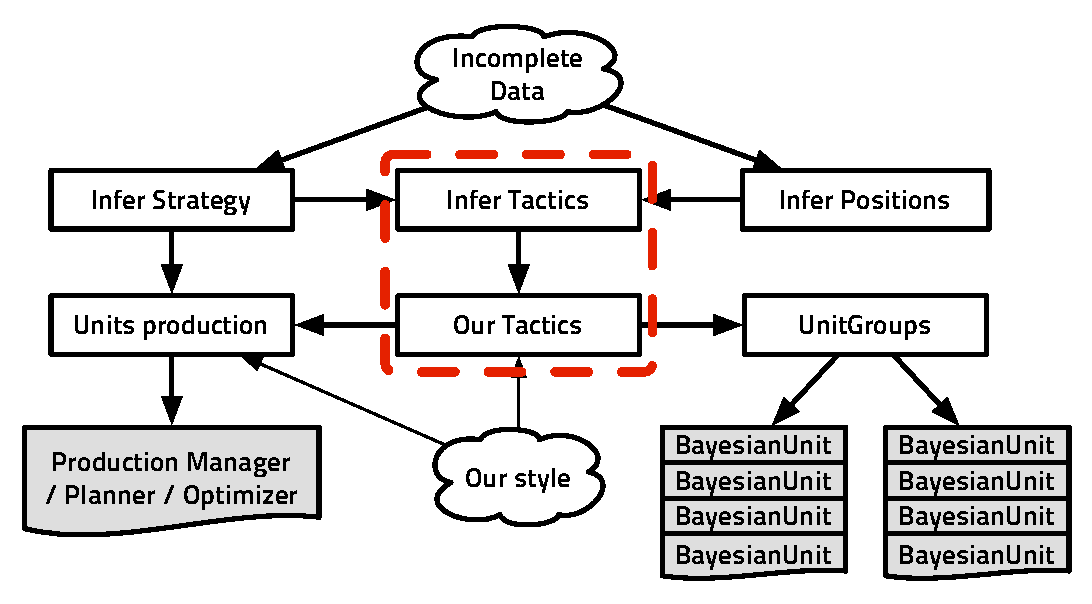
\includegraphics[width=13cm]{images/starcraft_bbq_concept_12-04-2012_TACTICS.pdf}
\end{center}
\label{fig:conceptTACTICS}
\caption{Information-centric view of the architecture of the bot, the part concerning this chapter is in the dotted rectangle}
\end{figure}
\begin{itemize}
\item Problem: choose which tactical actions/goals to persue, peform the action
\item Complexity: incompleteness/uncertainty problem, lot of low level information to handle, w.r.t. full and higher level information, simple.
\item State of the art: \citep{SORTS, Weber2010cr, Balla, CadenaG11}
\item Our take: low level heuristics that we learn to adapt to
\item Results: XXX
\item Conclusion and perspectives: still enabled for meta-game, and even in-game, adaptation. Could learn the action sequences of tactics from replays ($\approxeq$HMM).
\end{itemize}

